\section{Cache-Speicher}

\textbf{Hintergrund}
\begin{items}
	\item Lücke zwischen Verarbeitungs- (CPU) und Zugriffsgeschwindigkeit (DRAM) immer größer
	\item \underline{Lösung}: Hierarchische Anordnung verschiedener Speicher \\*
		\( \leadsto \) Ausgleich der unterschiedlichen Zugriffszeiten
	\item \underline{Strategien}:
	\begin{enumeration}
		\item \textbf{Cache-Speicher}: Kurze Zugriffszeiten \\*
			\( \leadsto \) Beschleunigung Prozessorzugriff
		\item \textbf{Virtueller Speicher}: Vergrößerung des tatsählich vorhandenen Hauptspeichers (z.B. bei gleichzeitiger Bearbeitung mehrerer Prozesse)
	\end{enumeration}
	\item Leistung abhängig von Eigenschaften der Speichertechnologien, Adressierung und Organisation
\end{items}
\begin{figure}[H]\centering\label{Speicherhierarchie}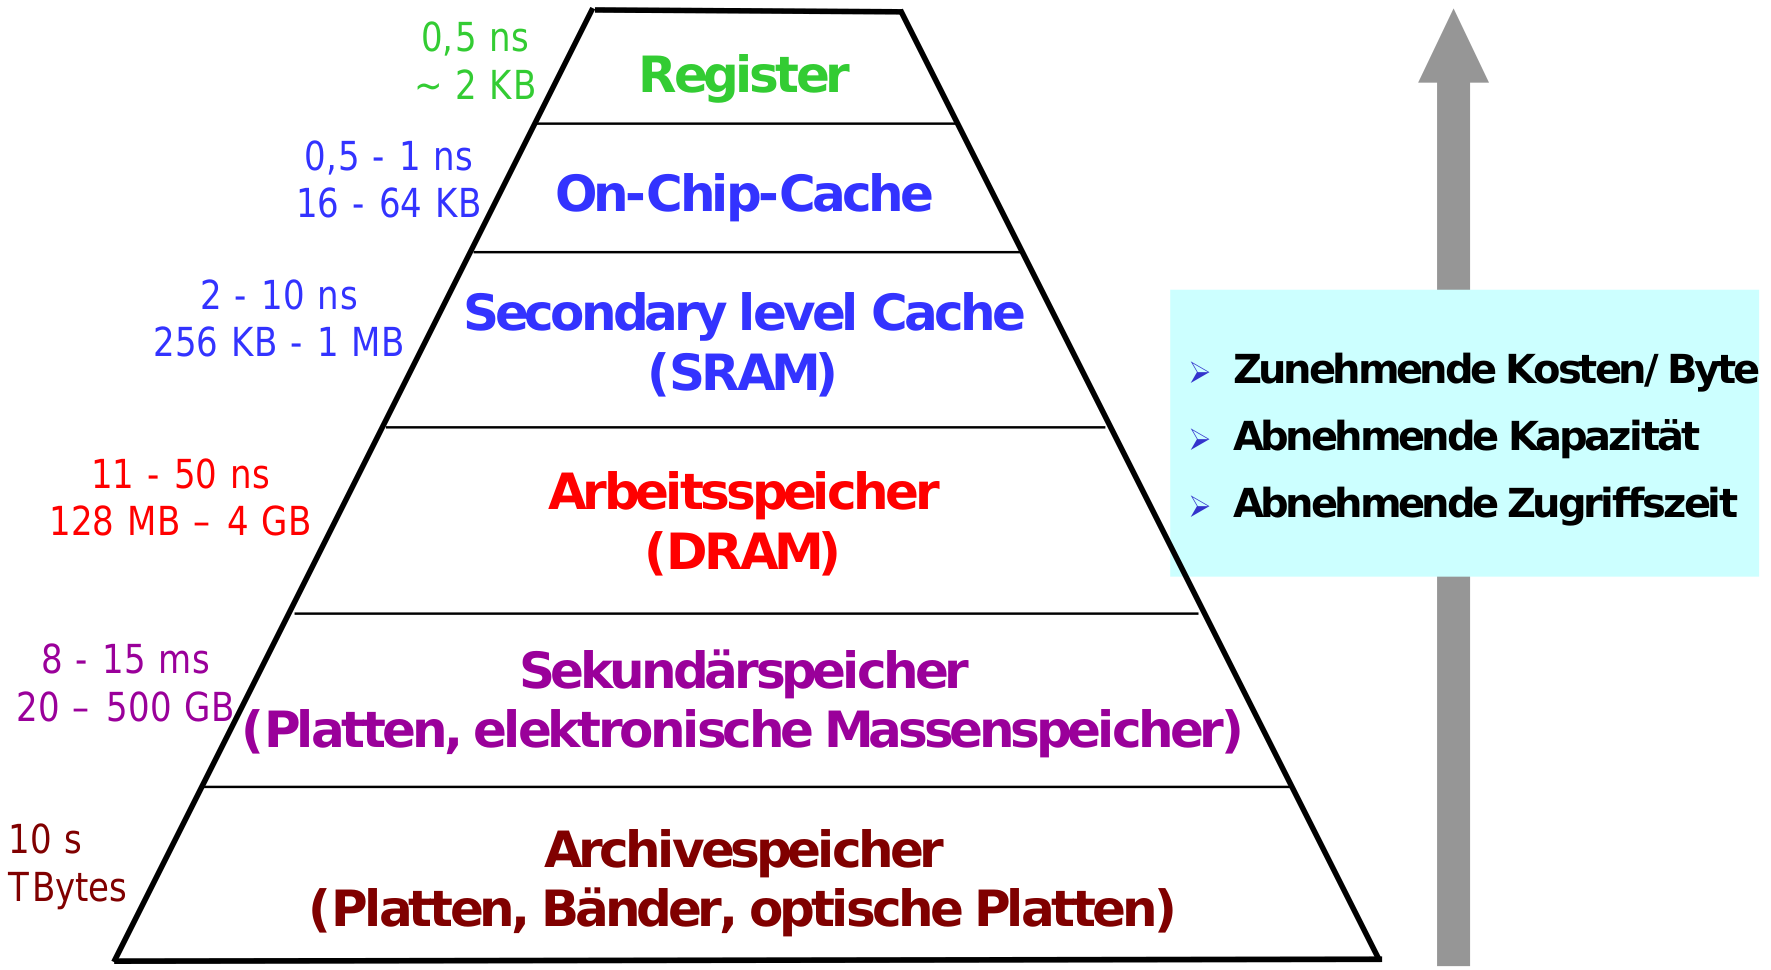
\includegraphics[width=0.33\textwidth]{Speicherhierarchie}\end{figure}

\newpage

\textbf{CPU-Cache}
\begin{items}
	\item kleiner, schneller Pufferspeicher
	\item speichert \emph{Kopien} von Hauptspeicherteilen, auf die mit hoher Wahrscheinlichkeit als nächstes zugegriffen wird
	\item Effizienz durch \emph{Lokalitätseigenschaft} von Programmen:
	\begin{enumeration}
		\item \textbf{zeitliche Lokalität}: zukünftig angesprochene Information mit hoher Wahrscheinlichkeit schon einmal angesprochen worden (z.B. Schleifen)
		\item \textbf{örtliche Lokalität}: zukünftig angesprochene Information mit hoher Wahrscheinlichkeit in Nähe des bisherigen Zugriffs (z.B. Arrays)
	\end{enumeration}
	\item \emph{Cache-Controller} lädt alle Daten in Cache, auf die Prozessor zugreift
	\item Daten werden aus Cache verdrängt, wenn sie nicht mehr benötigt werden
\end{items}

\textbf{Cache -- Funktionsweise}
\begin{items}
	\item \underline{Lesezugriff}: \( \mu \)P überprüft davor ob Datum in Cache steht \\*
		- \textbf{read hit}: Datum wird ohne Wartezyklen aus Cache geladen \\*
		- \textbf{read miss}: Datum wird mit Wartezyklen aus Arbeitsspeicher \\* \phantom{-} geladen und in Cache eingefügt
	\item \underline{Schreibzugriff}: \\*
		- \textbf{write miss}: Datum wird in DRAM und Cache geschrieben \\*
		- \textbf{write hit}: verschiedene Verfahren möglich
\end{items}

\textbf{Schreibzugriff -- Durchschreibverfahren}
\begin{items}
	\item Datum wird von CPU immer gleichzeitig in Cache- und Arbeitsspeicher geschrieben
	\item \underline{Vorteil}: Konsistenzgarantie zwischen Cache und DRAM
	\item \underline{Nachteil}: Schreibzugriffe benötigen immer langsame Zykluszeit von Hauptspeicher, belasten Systembus
\end{items}

\textbf{Schreibzugriff -- gepuffertes Durchschreibverfahren}
\begin{items}
	\item Verwendung von \emph{Schreib-Puffer}, der zu schreibende Daten temporär aufnimmt
	\item Daten werden dann automatisch von Cache-Controller in Hauptspeicher übertragen
\end{items}

\textbf{Schreibzugriff -- Rückschreibverfahren}
\begin{items}
	\item Datum wird von CPU nur in Cachespeicher geschrieben und durch spezielles Bit (\emph{dirty bit}) gekennzeichnet
	\item Arbeitsspeicher wird nur geändert, wenn \emph{dirty}-Datum aus Cache verdrängt wird
	\item \underline{Vorteil}: Alle Schreibzugriffe mit schneller Cache-Zykluszeit abwickelbar
	\item \underline{Nachteil}: Konsistenzprobleme zwischen Cache- und Hauptspeicher
\end{items}

\textbf{Konsistenzprobleme}
\begin{items}
	\item Andere Systemkomponenten (z.B. DMA-Controller) finden ggf "`veraltete Daten"' in DRAM vor, die von CPU längst geändert wurden
	\item Andere Systemkomponenten können Daten in Hauptspeicher ändern, während CPU noch mit alten Daten aus Cache arbeitet
	\item \( \leadsto \) aufwendige Verfahren bei Cache-Steuerung zur Inkonsistenzvermeidung erforderlich
\end{items}

\textbf{Begriffe}
\begin{items}
	\item \underline{Hit-Rate}: = Anzahl Treffer pro Anzahl Zugriffe
	\item \underline{Mittlere Zugriffszeit}: \\*
		\( t_{\text{access}} = (\text{Hit-Rate})t_\text{hit}+(1-\text{Hit-Rate})t_\text{miss} \)
\end{items}

\textbf{Cache-Speicher -- Aufbau}
\begin{items}
	\item Besteht aus drei Teilen:
	\begin{enumeration}
		\item \textbf{Datenspeicher}: im Cache abgelegte Daten
		\item \textbf{Adressspeicher}: Adresse dieses Datums im RAM
		\item \textbf{Statusbits}: Geben an, ob Informationen gültig sind
	\end{enumeration}
	\item Zusammen: \emph{cache-line}
	\item \underline{Komparator}: ermittelt, ob zu Adressbus gehörendes Datum in Cache abgelegt ist
\end{items}

\textbf{Cache-Speicher -- Organisation}
\begin{items}
	\item \underline{Problem}: Wie feststellen, ob Daten im Cache sind? Wie können diese gefunden werden?
	\item Techniken für Adressvergleich:
	\begin{enumeration}
		\item \textbf{voll-assoziativer Cache}
		\item \textbf{direct mapped cache}
		\item \textbf{n-way set associative cache}
	\end{enumeration}
\end{items}

\textbf{Cache-Speicher -- voll-assoziativer Cache}
\begin{items}
	\item Gesamter Hauptspeicher wird auf gesamten Cache abgebildet
	\item \( \leadsto \) Jeder aus dem Hauptspeicher gecachte Wert kann an jeder Stelle im Cache stehen
	\item \underline{Vorteile}: \\*
		- beliebiges Ablegem \\*
		- optimale Cache-Ausnutzung
	\item \underline{Nachteile}: \\*
		- hoher HW-Aufwand (ein Vergleicher pro Cachezeile) \\*
			\phantom{-} \( \leadsto \) nur für sehr kleine Caches realisierbar\\*
		- große Flexibilität erfordert weitere HW, die \\* \phantom{-} Ersetzungsstrategie realisiert
\end{items}
\begin{figure}[H]\centering\label{VollAssoziativerCache}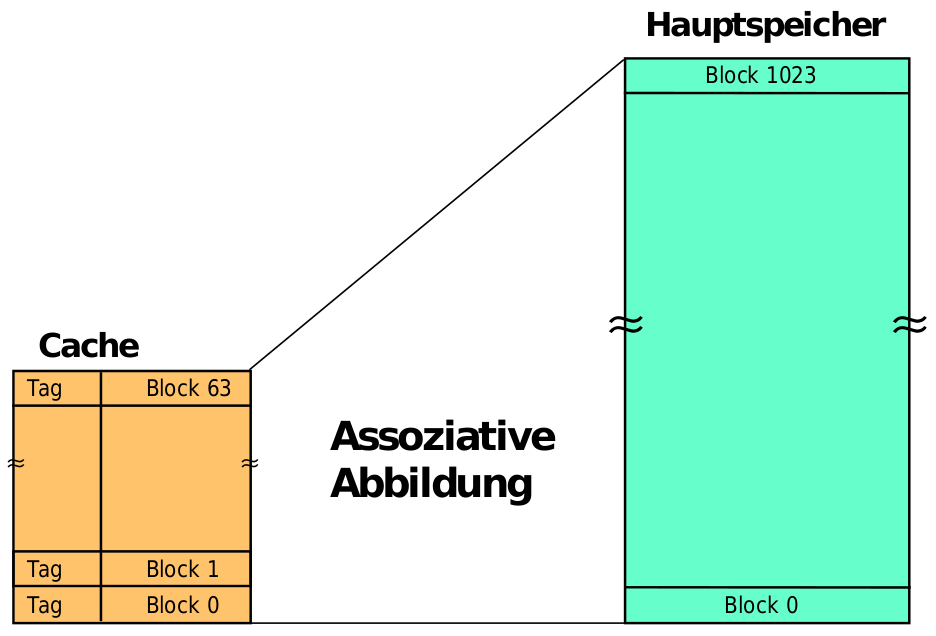
\includegraphics[width=0.2\textwidth]{VollAssoziativerCache}\end{figure}

\textbf{Cache-Speicher -- direct mapped-Cache}
\begin{items}
	\item jede Hauptspeicherstelle erhält eindeutigen, festen Cacheplatz
	\item \underline{Vorteile}: \\*
		- Geringer HW-Aufwand (ein Vergleicher für alle Tags) \\*
		- schneller Zugriff, da Tag-Feld parallel zu zugehörigem Block gelesen werden kann \\*
		- keine Ersetzungsstrategie erforderlich
	\item \underline{Nachteile}: \\*
		- ständige Konkurrenz der Blöcke, obwohl andere Blöcke frei \\* \phantom{-} sein können \\*
		- bei abwechselndem Zugriff auf zwei Speicherblöcke aus \\* \phantom{-} gleichem Index-Teil entsteht laufendes Überschreiben \\* \phantom{-} (aka \emph{flattern}, \emph{trashing})
\end{items}
\begin{figure}[H]\centering\label{DirectMappedCache}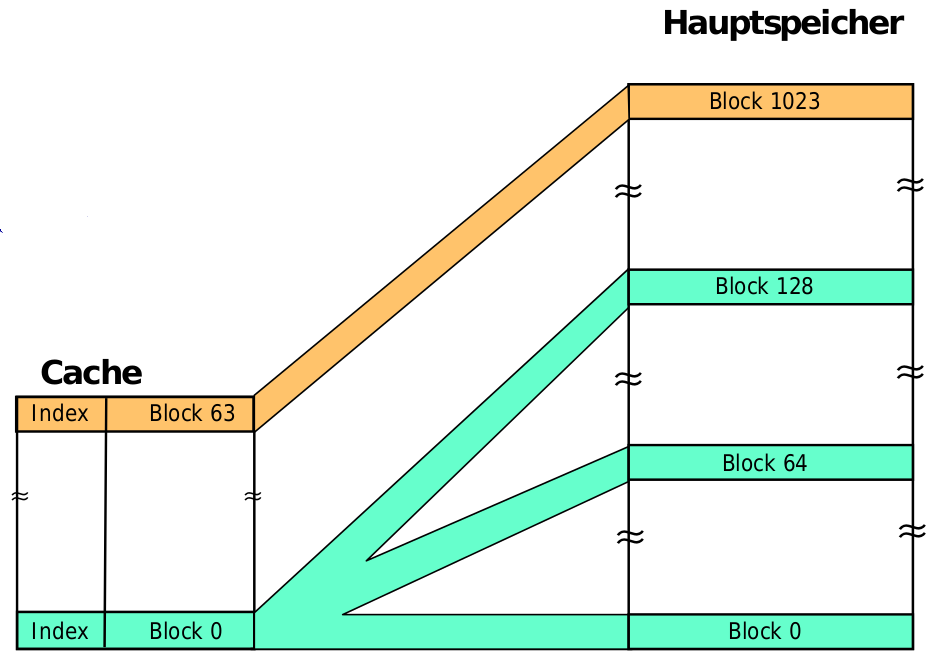
\includegraphics[width=0.2\textwidth]{DirectMappedCache}\end{figure}

\textbf{Cache-Speicher -- N-way set associative-Cache}
\begin{items}
	\item Mehrere Cache-Zeilen (z.B. 2) werden zu Sets zusammengefasst
	\item Kompromiss zwischen direct mapped- und vollassoziativem Cache
	\item Berbesserte Trefferrate durch Auswahlmöglichkeit
	\item \underline{Ersetzungsstrategie}: \\*
		- \textbf{zyklisch}: erster gespeicherter Eintrag wird als erster verdrängt \\* \phantom{-} (FIFO) \\*
		- \textbf{LRU} (\emph{last recently used}): am längsten unbenutzter Eintrag \\* \phantom{-} wird verdrängt \\*
		- \textbf{zufällig}
\end{items}

\textbf{Cache-Speicher -- Ersetzungsstrategien}
\begin{items}
	\item gibt an, welcher Cachespeicherteil nach cache miss durch neu geladene Speicheroption überschrieben werden soll
	\item ist nur bei voll/n-fach-satzassoziativer Cachespeicherorganisation nötig
	\item \underline{LRU} (\emph{last recently used}): am längsten nicht benutzte Speicherportion wird ersetzt (schwer in HW umzusetzen, deswegen meist nur Pseudo-LRU)
\end{items}

\textbf{Ursachen für Fehlzugriffe}
\begin{items}
	\item \underline{Erstzugriff} (\emph{compulsory}): Bei Erstzugriff auf Cache-Block ist dieser noch nicht im Cache und muss geladen werden \\*
	- Kaltstartfehlzugriffe (\emph{cold start misses}) \\*
	- Erstbelegungsfehlzugriffe (\emph{first reference misses})
	\item \underline{Kapazität} (\emph{capacity}): Falls Cache-Speicher nicht alle benötigten Cache-Blöcke aufnehmen kann müssen Cache-Blöcke verdrängt (und ggf später neu geladen) werden
	\item \underline{Konlfikt} (\emph{conflict}): Cache-Block wird verdrändt und später neu geladen, falls zu viele Cache-Blöcke auf selben Satz abgebildet werden \\*
	- Kollisionsfehlzugriffe (\emph{collision misses}) \\*
	- Interferenzfehlzugriffe (\emph{interference misses})
\end{items}

\textbf{Trefferquotenmaximierung}
\begin{items}
	\item \underline{Sehr kleine Cachespeicher} (32-128 Einträge): Voll-assoziativ
	\item \underline{Größere Cachespeicher}: Trend zu Direct Mapped oder 2-8-fach-assoziativ
\end{items}

\textbf{Systembusanbindung}
\begin{items}
	\item \underline{Cache-Controller}: Tag-RAM, Steuerung, Tag-Komparator \\*
		- muss sehr schnell sein \( \leadsto \) auf Chip integriert \\*
		- übernimmt Steuerung der Treiber zum Systembus \\* \phantom{-} (Systembuszugriff nur bei Cache-Miss, ansonsten ist \\* \phantom{-} Systembus für andere Komponenten frei) \\*
		- sendet Systembussignale zur Wartezykleneinführung bei \\* \phantom{-} Cache-Miss (\code{READY}, \code{HOLD}, \code{HOLDA},\dots)
	\item \underline{Cachespeicher}: separat aus SRAM-Bausteinen aufgebaut
\end{items}

\textbf{Cache -- Hierarchien}
\begin{items}
	\item \underline{First-Level Cache} (\emph{on-chip cache}): Auf Prozessor-Chip \\*
		- oft in \textbf{Befehlscache} und \textbf{Datencache} unterteilt
	\item \underline{Secondary-Level Cache} (\emph{on-board cache}) \\*
		- kann parallel zu Hauptspeicher an Bus angeschlossen werden \\* \phantom{-} (\emph{look-aside cache}) \( \leadsto \) schnelles Nachladen bei first-level-miss
\end{items}
\begin{figure}[H]\centering\label{CacheHierarchie}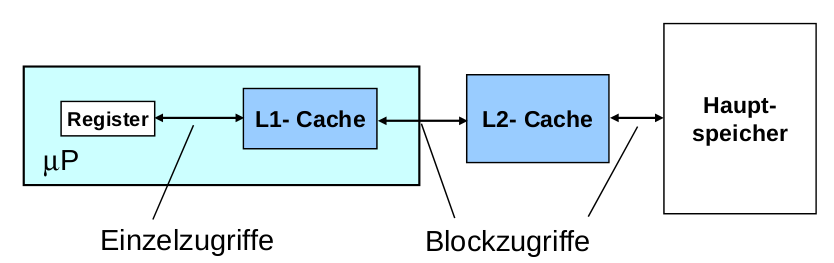
\includegraphics[width=0.33\textwidth]{CacheHierarchie}\end{figure}

\textbf{Cache -- Kohärenzproblem}
\begin{items}
	\item \underline{Kohärenz}: korrektes Voranschreiten des Systemzustands durch abgestimmtes Zusammenwirken der Einzelzustände
	\item \underline{Konsistenz}: alle Kopien eines Hauptspeicherdatums in verschiedenen Cachespeichern identisch \\* \( \leadsto \) \textbf{Kohärenz-Sicherstellung}
\end{items}

\textbf{Bus-Schnüffeln (Snooping)}
\begin{items}
	\item verwendet bei Mehrprozessorsystemen mit lokalem Cache pro Prozessor und gemeinsamen Hauptspeicher
	\item \underline{Schnüffel-Logik}: jeder Prozessor hört an Bus mit, wenn andere Prozessoren Adressen auf Bus legen \\* \( \leadsto \) Vergleich mit den im lokalen Cache gespeicherten Daten
\end{items}

\textbf{Snooping -- Verfahren}
\begin{items}
	\item \underline{Schreibzugriff} auf dieselbe Adresse: \\*
		- Cache-Block für ungültig erklären (\emph{write-invalidate}) \\*
		- Cache-Block aktualisieren (\emph{write-update})
	\item \underline{Lesezugriff} auf dieselbe Adresse mit modifiziertem Datum \\*
		\( \leadsto \) Cache-Controller legt \emph{snoop status signal} (\code{SSTAT}) auf Bus
	\begin{enumeration}
		\item Prozessor, der Adresse auf Bus gelegt hat, unterbricht Bustransaktion
		\item schnüffelnder Cache-Controller übernimmt Bus und schreibt Cacheblock in Hauptspeicher
		\item erneute Ausführung der Bustransaktion
	\end{enumeration}
\end{items}